% case name
\chapter{Supertab}
%
%
% - Purpose & Description:
%     These first two parts give reader short details about the test case,
%     the physical phenomena involved, the geometry and specify how the numerical solution will be validated
\section{Purpose}
This example illustrates the conversion from a mesh file generated with
SUPERTAB to a Serafin file.
%
\section{Description}
This mesh has been realised with "quadrangle" elements. Then, it is no use to
eliminate the overstressed triangles.\\
Knowing that SUPERTAB software does not understand the bathymetry and that the \stbtel
computation is made without any bottom topography files, there is consequently no variable
BOTTOM on the final mesh file.\\
In the steering file, the user indicates the name of the files to be used, specifies the used
mesh software and finally push on the elimination of the backward dependencies. (The
\telemac{2D} computation will be done on a vector machine with 128 bytes vector length).

%
% - Physical parameters:
%     This part specifies details all the physical parameters
%\subsection{Physical parameters}
%
% Experimental results (if needed)
%\subsection{Experimental results}
%
% bibliography can be here or at the end
%\subsection{Reference}
%
% Section for computational options
%\section{Computational options}
%
% - Mesh:
%     This part describes the mesh used in the computation
%\subsection{Mesh}
%
% - Initial and boundary conditions:
%     This part details both initial and boundary conditions used to simulate the case
%\subsection{Initial and boundary conditions}
%
% - Numerical parameters:
%     This part is used to specify the numerical parameters used
%     (adaptive time step, mass-lumping when necessary...)
%\subsection{Numerical parameters}
%
% - Results:
%     We comment in this part the numerical results against the reference ones,
%     giving understanding keys and making assumptions when necessary.
\section{Results}
The resulted mesh is shown in figure \ref{fig:supertab:mesh}:
\begin{figure}[H]%
\begin{center}
%
  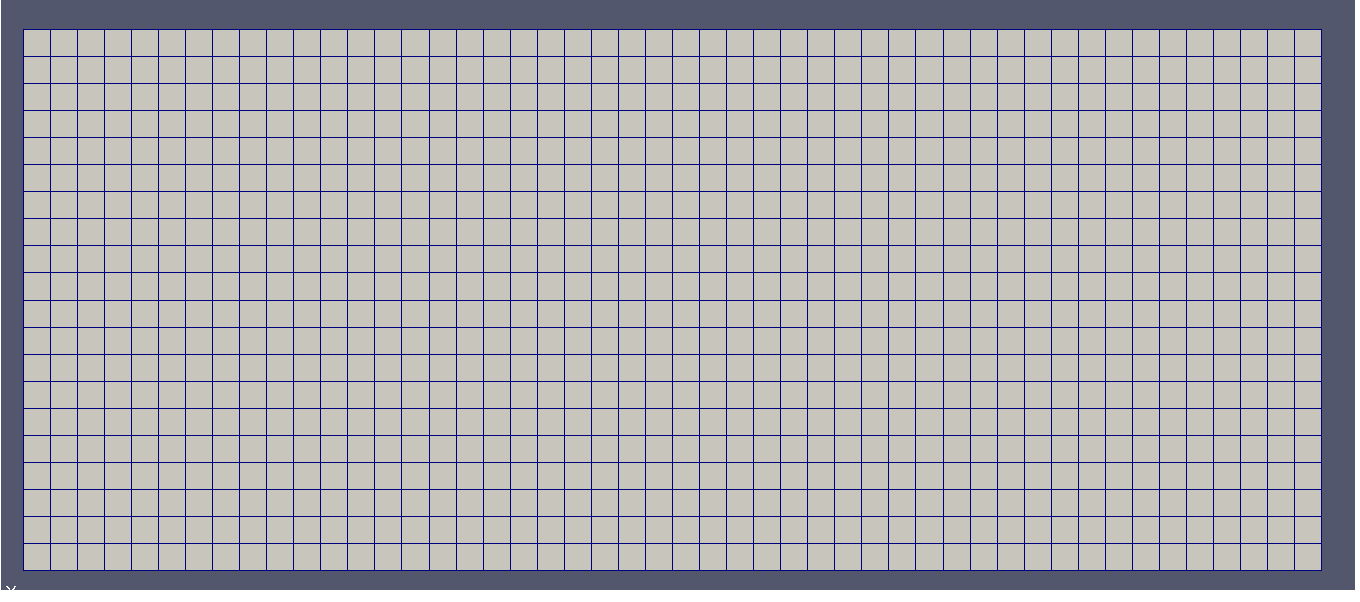
\includegraphics[width=0.9\textwidth]{mesh}
%
\end{center}
\caption
{The mesh}
\label{fig:supertab:mesh}
\end{figure}
%
% bibliography
%\section{Reference}
